%==============================================================================
% tento soubor pouzijte jako zaklad
% this file should be used as a base for the thesis
% (c) 2008 Michal Bidlo
% E-mail: bidlom AT fit vutbr cz
% Šablonu upravil / template edited by: Ing. Jaroslav Dytrych, dytrych@fit.vutbr.cz
%==============================================================================
% kodovaní: UTF-8 (zmena prikazem iconv, recode nebo cstocs)
% encoding: UTF-8 (you can change it by command iconv, recode or cstocs)
%------------------------------------------------------------------------------
% zpracování / processing: make, make pdf, make clean
%==============================================================================
% Soubory, které je nutné upravit: / Files which have to be edited:
%   projekt-20-literatura-bibliography.bib - literatura / bibliography
%   projekt-01-kapitoly-chapters.tex - obsah práce / the thesis content
%   projekt-30-prilohy-appendices.tex - přílohy / appendices
%==============================================================================
\documentclass[]{fitthesis} % bez zadání - pro začátek práce, aby nebyl problém s překladem
%\documentclass[english]{fitthesis} % without assignment - for the work start to avoid compilation problem
%\documentclass[zadani]{fitthesis} % odevzdani do wisu - odkazy jsou barevné
%\documentclass[english,zadani]{fitthesis} % for submission to the IS FIT - links are color
%\documentclass[zadani,print]{fitthesis} % pro tisk - odkazy jsou černé
%\documentclass[english,zadani,print]{fitthesis} % for the print - links are black
% * Je-li prace psana v anglickem jazyce, je zapotrebi u tridy pouzit 
%   parametr english nasledovne:
%   If thesis is written in english, it is necessary to use 
%   parameter english as follows:
%      \documentclass[english]{fitthesis}
% * Je-li prace psana ve slovenskem jazyce, je zapotrebi u tridy pouzit 
%   parametr slovak nasledovne:
%      \documentclass[slovak]{fitthesis}

% Základní balíčky jsou dole v souboru šablony fitthesis.cls
% Basic packages are at the bottom of template file fitthesis.cls
%zde muzeme vlozit vlastni balicky / you can place own packages here

%---rm---------------
\renewcommand{\rmdefault}{lmr}%zavede Latin Modern Roman jako rm / set Latin Modern Roman as rm
%---sf---------------
\renewcommand{\sfdefault}{qhv}%zavede TeX Gyre Heros jako sf
%---tt------------
\renewcommand{\ttdefault}{lmtt}% zavede Latin Modern tt jako tt

% vypne funkci šablony, která automaticky nahrazuje uvozovky,
% aby nebyly prováděny nevhodné náhrady v popisech API apod.
% disables function of the template which replaces quotation marks
% to avoid unnecessary replacements in the API descriptions etc.
\csdoublequotesoff

% =======================================================================
% balíček "hyperref" vytváří klikací odkazy v pdf, pokud tedy použijeme pdflatex
% problém je, že balíček hyperref musí být uveden jako poslední, takže nemůže
% být v šabloně
% "hyperref" package create clickable links in pdf if you are using pdflatex.
% Problem is that this package have to be introduced as the last one so it 
% can not be placed in the template file.
\ifWis
\ifx\pdfoutput\undefined % nejedeme pod pdflatexem / we are not using pdflatex
\else
  \usepackage{color}
  \usepackage[unicode,colorlinks,hyperindex,plainpages=false,pdftex]{hyperref}
  \definecolor{links}{rgb}{0.4,0.5,0}
  \definecolor{anchors}{rgb}{1,0,0}
  \def\AnchorColor{anchors}
  \def\LinkColor{links}
  \def\pdfBorderAttrs{/Border [0 0 0] }  % bez okrajů kolem odkazů / without margins around links
  \pdfcompresslevel=9
\fi
\else % pro tisk budou odkazy, na které se dá klikat, černé / for the print clickable links will be black
\ifx\pdfoutput\undefined % nejedeme pod pdflatexem / we are not using pdflatex
\else
  \usepackage{color}
  \usepackage[unicode,colorlinks,hyperindex,plainpages=false,pdftex,urlcolor=black,linkcolor=black,citecolor=black]{hyperref}
  \definecolor{links}{rgb}{0,0,0}
  \definecolor{anchors}{rgb}{0,0,0}
  \def\AnchorColor{anchors}
  \def\LinkColor{links}
  \def\pdfBorderAttrs{/Border [0 0 0] } % bez okrajů kolem odkazů / without margins around links
  \pdfcompresslevel=9
\fi
\fi
% Řešení problému, kdy klikací odkazy na obrázky vedou za obrázek
% This solves the problems with links which leads after the picture
\usepackage[all]{hypcap}

% Informace o práci/projektu / Information about the thesis
%---------------------------------------------------------------------------
\projectinfo{
  %Prace / Thesis
  project=BP,            %typ prace BP/SP/DP/DR  / thesis type (SP = term project)
  year=2017,             %rok odevzdání / year of submission
  date=\today,           %datum odevzdani / submission date
  %Nazev prace / thesis title
  title.cs={Radarový výškoměr pro ultralehký letoun},  %nazev prace v cestine ci slovenstine (dle zadani) / thesis title in czech language (according to assignment)
  title.en={Radar Altimeter for Ultralight Aircraft}, %nazev prace v anglictine / thesis title in english
  %Autor / Author
  author={Jiří Zahradník},   %cele jmeno a prijmeni autora / full name and surname of the author
  author.name={Jiří},   %jmeno autora (pro citaci) / author name (for reference) 
  author.surname={Zahradník},   %prijmeni autora (pro citaci) / author surname (for reference) 
  %author.title.p=Bc., %titul pred jmenem (nepovinne) / title before the name (optional)
  %author.title.a=PhD, %titul za jmenem (nepovinne) / title after the name (optional)
  %Ustav / Department
  department=UPGM, % doplnte prislusnou zkratku dle ustavu na zadani: UPSY/UIFS/UITS/UPGM
  %                  fill in appropriate abbreviation of the department according to assignment: UPSY/UIFS/UITS/UPGM
  %Skolitel / supervisor
  supervisor=Lukáš Maršík, %cele jmeno a prijmeni skolitele / full name and surname of the supervisor
  supervisor.name={Lukáš},   %jmeno skolitele (pro citaci) / supervisor name (for reference) 
  supervisor.surname={Ing.~Maršík},   %prijmeni skolitele (pro citaci) / supervisor surname (for reference) 
  supervisor.title.p={Ing.},   %titul pred jmenem (nepovinne) / title before the name (optional)
  supervisor.title.a={},    %titul za jmenem (nepovinne) / title after the name (optional)
  %Klicova slova, abstrakty, prohlaseni a podekovani je mozne definovat 
  %bud pomoci nasledujicich parametru nebo pomoci vyhrazenych maker (viz dale)
  %Keywords, abstracts, declaration and acknowledgement can be defined by following 
  %parameters or using dedicated macros (see below)
  %===========================================================================
  %Klicova slova / keywords
  %keywords.cs={Klíčová slova v českém jazyce.}, %klicova slova v ceskem ci slovenskem jazyce
  %                                              keywords in czech or slovak language
  %keywords.en={Klíčová slova v anglickém jazyce.}, %klicova slova v anglickem jazyce / keywords in english
  %Abstract
  %abstract.cs={Výtah (abstrakt) práce v českém jazyce.}, % abstrakt v ceskem ci slovenskem jazyce
  %                                                         abstract in czech or slovak language
  %abstract.en={Výtah (abstrakt) práce v anglickém jazyce.}, % abstrakt v anglickem jazyce / abstract in english
  %Prohlaseni / Declaration
  %declaration={Prohlašuji, že jsem tuto bakalářskou práci vypracoval samostatně pod vedením pana ...},
  %Podekovani (nepovinne) / Acknowledgement (optional)
  %acknowledgment={Zde je možné uvést poděkování vedoucímu práce a těm, kteří poskytli odbornou pomoc.} % nepovinne
  %acknowledgment={Here it is possible to express thanks to the supervisor and to the people which provided professional help.} % optional
}

%Abstrakt (cesky, slovensky ci anglicky) / Abstract (in czech, slovak or english)
\abstract[cs]{V~této bakalářské práci se~autor zabývá návrhem a částečnou implementací radarového výškoměru. V této práci je kladen důraz na modulární architekturu a~proto je tento výškoměr navržen jako soubor samostatných modulů komunikujících pomocí BSD schránek. Implementace programového vybavení je v~C++ a~pro generování zvuku je použita knihovna PulseAudio. Dále je zde řešena bezpečnost mezivláknové fronty a~zásobníku pomocí třídy implementované jako šablona pro~zachování jednoduchosti a~obecnosti pro~další využití.} 
\abstract[en]{In this bachelor thesis author designs a~radar altimeter. In~this thesis the~emphasis is placed onto modular architecture andthat is why this altimeter is designed as a~group of~independent modules communicating through BSD sockets. Software implementation is made in~C++ and~for sound generator is used library PulseAudio. Next topic is multithreading safety implementation of~queue and~stack which was made by template class to keep simplicity and generality.}

%Klicova slova (cesky, slovensky ci anglicky) / Keywords (in czech, slovak or english)
\keywords[cs]{radar, výškoměr, PulseAudio, C++, vícevláknové zpracování, BSD schránky, avionika, generování zvuku, vestavěné systémy, Xilinx Zynq, FPGA, USB zvuková karta, přistání}
\keywords[en]{radar, altimeter, PulseAudio, C++, multithreading, BSD sockets, avionics, sound generating, embedded systems, Zynq, FPGA, USB soundcard, landing}

%Prohlaseni (u anglicky psane prace anglicky, u slovensky psane prace slovensky)
%Declaration (for thesis in english should be in english)
\declaration{Prohlašuji, že jsem tuto bakalářskou práci vypracoval samostatně pod vedením pana Ing.~Lukáše Maršíka.
Uvedl jsem všechny literární prameny a~publikace, ze~kterých jsem čerpal.}

% \declaration{Hereby I declare that this bachelor's thesis was prepared as an original author’s work under the supervision of Mr. X
% The supplementary information was provided by Mr. Y
% All the relevant information sources, which were used during preparation of this thesis, are properly cited and included in the list of references.}

%Podekovani (nepovinne, nejlepe v jazyce prace) / Acknowledgement (optional, ideally in the language of the thesis)
\acknowledgment{Tímto chci poděkovat mému vedoucímu, panu Ing.~Lukáši Maršíkovi za odborné vedení práce a~kolegům z práce za poskytnutí doplňujících informací.}
%\acknowledgment{Here it is possible to express thanks to the supervisor and to the people which provided professional help
%(external submitter, consultant, etc.).}

% řeší první/poslední řádek odstavce na předchozí/následující stránce
% solves first/last row of the paragraph on the previous/next page
\clubpenalty=10000
\widowpenalty=10000

\begin{document}
  % Vysazeni titulnich stran / Typesetting of the title pages
  % ----------------------------------------------
  \maketitle
  % Obsah
  % ----------------------------------------------
  \tableofcontents
  
  % Seznam obrazku a tabulek (pokud prace obsahuje velke mnozstvi obrazku, tak se to hodi)
  % List of figures and list of tables (if the thesis contains a lot of pictures, it is good)
\ifczech
  \renewcommand\listfigurename{Seznam obrázků}
\fi
\ifslovak
  \renewcommand\listfigurename{Zoznam obrázkov}
\fi

  % \listoffigures
\ifczech
  \renewcommand\listtablename{Seznam tabulek}
\fi
\ifslovak
  \renewcommand\listtablename{Zoznam tabuliek}
\fi

  % \listoftables 

  % vynechani stranky v oboustrannem rezimu
  % Skip the page in the two-sided mode
  \iftwoside
    \cleardoublepage
  \fi

  % Text prace / Thesis text
  % ----------------------------------------------
  %=========================================================================
% (c) Michal Bidlo, Bohuslav Křena, 2008

\newtheorem{definice}{Definice}

\chapter{Úvod}\label{uvod}
	Výškoměr je jedím z nepostradatelných přístrojů pro navigaci za letu. Je důležité aby fungoval správně ve~všech situacích, jelikož~chyba v~měření může znamenat havárii letadla. V~lepším případě dojde "pouze" ke~škodám na~majetku, v~horším případě může dojít i~ke~ztrátám na~životech. Plní nezastupitelnou úlohu, díky níž mohou piloti bezpečně létat i~za~špatné viditelnosti.
	
	\section{Motivace}\label{uvod::motivace}
		Motivace pro tuto práci je zvýšení bezpečnosti a~ulehčení výcviku začínajicích pilotů. Jde hlavně o~ulehčení výuky přistání, která začátečníkovi může způsobovat poťíže. Jedná se primárně o~výuku dosednutí(anglicky "flare"), kdy musí student stáhnout výkon motoru a~přitáhnutím uvést letoun do~horizontálního letu, ideálně několik centimetrů nad dráhou. Student pomalu přitahuje knipl, tímto~zvyšuje úhel náběhu a~letadlo postupně zpomaluje. V~okamžiku, kdy je úhel náběhu příliš velký a~rychlost letadla moc nízká, křídla ztratí vztak a~letadlo dosedne na dráhu. Pokud student udžuje letadlo v~horizontálním letu nad dráhou ve~velké výšce, může být dosednutí tvrdší, než na~které~je stavěn podvozek, a~může dojít k~poškození podvozku či~zranění posádky i~cestujících.
	
	\section{Cíle}\label{uvod::cile}
		Prvním cílem této práce je úvod do~problematiky týkající se~radarů. Čtenáři budou přiblíženy rozdíly mezi jednotlivými typy radarů, principy jejich fungování a~technologiemi, které za~nimi stojí. Druhým cílem je popis problému výuky přistání a~důvod pro zadání této práce, jakožto i~jejího řešení. Třetím cílem je návrh takového systému, který~splní veškeré požadavky na bezpečnost letového provozu na letištích, zvýší bezpečnost výuky přistání a~samozřejmě zjednodušší samotnou výuku. V neposlední řadě je samotná implementace již zmíněného systému a~jeho integrace do letadla. Nakonec je třeba systém jako celek otestovat a~zajistit, že bude bezchybně fungovat za~jakýchkoliv podmínek. V~případě, že bude systém funkční, je možnost jej rozšířit a~aplikovat v~komerční praxi. 

\chapter{Teoretická část}
	\section{Fáze přistání}
		Letadlo, které~vzlétne, se musí dostat zpět na~zem rozumným a~hlavně bezpečným způsobem. Není žádoucí aby letadlo i~pasažéři byli na jedno použití. Bezpečné přistání je nejdůležitější fází letu.\par
		Když se blíže podíváme na přistání, je to doslova řízený pád. Letadlo ztrácí výšku a~rychlost aby~bezpečně dosedlo na zem a~je zde malý prostor chybovat. Proto je kladen velký důraz na výuku a~správné naučení přístávání. Přistání lze rozdělit do několika fází\cite{landingPhases}:
		
		\begin{enumerate}
			\item Závěrečné přiblížení (Final approach) - Během této fáze pilot musí udržovat přibližovací rychlost danou výrobcem letadla a~letět po kurzu osy dráhy pod sklonem určeným přibližovacími pravidly(glidepath).
			Během této fáze pilot uvádí letoun do přistávácí konfigurace.
			
			\item Výběh (zeptat se prof Zemcika na spravny cesky preklad Flare) - Když se pilot přibližuje k~dráze, musí přitáhnout knipl, tím zvýší úhel náběhu a~zpomalení stroje. Letadlo je závislé na rychlosti proudění vzduchu okolo křídel. Když je proud vzduchu příliš pomalý a~úhel náběhu nestíhá kompenzovat ztrátu vztlaku, letadlo se dostane do pádu. Pilotovým úkolem v~této fázi letu je s~vypnutým motorem udržovat letadlo ve vodorovném letu těsně nad dráhou, na kterou~pak dítky ztrátě vztlaku dosedne. Je důležité, aby letadlo bylo těsně nad dráhou, čím výše se v~okamžiku ztráty vztalu letadlo nachází, tím tvrdší přistání může čekat.
			
			\item Dosednutí a~rolování (Touchdown and taxi) - Po dosednutí pilot zpomalí letadlo na požadovanou rychlost pro rolování a~roluje na místo určené řídícím na věži. 
		\end{enumerate}
		
	\section{Historie výškoměrů}\label{teorie::historieVyskomeru}
		Barometry byly lidstvu známy již od~17. století, tyto bohužel obsahovaly vodu. Aby mohl být tlak vzduchu úspěšně změřen, barometr vyžadoval cca 10 metrů vysokou trubici. Avčak italskému matematikovi a~fyzikovi Evangelistovi Torricellimu se podařilo zkrátít délku trubice na 80cm nahrazením vody rtutí, která je cca třináctkrát hustší než voda. I přez své relativně malé rozměry je tento barometr pořád příliž velký pro masové rozšíření. Za další minimalizaci přístroje je zodpovědný francouzský vědec Lucien Vidi, který vynalez aneroidní barometr, přezdívaný aneroid\cite{history::aneroid}.\par
		
		V roce 1903 bratři Wrightové uskutečnili první řízený motorový let. Trval jen chvíli, ale~byl to~přelom v~technologii dopravy. Začala éra letectví. Za první světové války, kdy došlo k~prvnímu masivnímu rozšíření letadel,  ať~již k~průzkumným účelům, bombardování nebo~vzdušným soubojům byli piloti omezeni počasím a~za špatného počasí nemohli létat, jelikož neexistovala technologie, která by umožnila pilotovi nespoléhat pouze na svůj zrak a~navigovat za letu i~jinak, než~pouze vizuálně. Toto vedlo ke~snahám vyvinout systém, který~by~umožňoval navigaci za~jakýchkoliv podmínek. Za~jasného slunečného počasí nebo třeba v~bouřce.\par

		Proto se začaly přesouvat navigační přístroje z kapes a~rukou pilotů na~přístrojovou desku. Postupem času se přidávaly další a další přístroje. Jeden z přístrojů byl i~výše zmíněný aneroid.  Díky své konstrukci a~velikosti je odolnější vůči fyzickému poškození než~rtuťové barometry a~nezabírá tolik místa na~přístrojové desce. Aneroidy nebyly kalibrovány na~tlak vzduchu, ale~na~nadmořskou výšku. Nevýhodou těchto barometrů je jejich nepřesnost. Tyto barometry byly kalibrovány na~AMSL(height above mean sea level), takže neukazovaly přesnou výšku nad terénem, ale~nad mořem. Problém byl vyřešen přidáním možnosti ruční kalibrace, kdy se nastavila referenční nula na zemi před vzletem letadla. 
		Na obrázku \ref{uvod::historieVyskomeru::kokpit} můžeme vidět typ výškoměru, který~byl používán německých letadlech během 2.světové války s~kolečkem umožňujícím nastavení referenční hodnotu země. 
		
		\begin{figure}[h]
			\begin{center}
				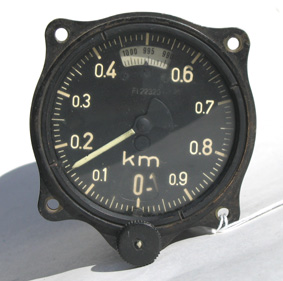
\includegraphics[scale=0.8]{obrazky-figures/109Altimeter.jpg}
				\caption{Německý výškoměr z 2.světové války\protect\footnotemark}
				\label{uvod::historieVyskomeru::kokpit}
			\end{center}
		\end{figure}
		\footnotetext{zdroj: \url{http://www.warbirdsite.com/}}
		
		V současnosti se ke~zjištění letové hladiny moderních letadel používá GPS. Systém GPS, narozdíl od~aneroidu není závislý na~počasí či~povětrnostních podmínkách a~udává přesnou výšku, souřadnice, kurz, stoupání/klesání a rychlost. Aneroidy se však i~nadále používají pro svou jednoduchost a~spolehlivost.
		
		\subsection{Existující radarové výškoměry}
			Radarové výškoměry nejsou žádná novinka. Dnes jsou využívány v~letectví ale i~pro vědecké účely.
			V letectví jsou hlavní součástí GPWS(Ground Proximity Warning System) kde~se používá jako absolutní výškoměr(měří vzdálenost letadla od~zemského povrchu). Teto systém byl rozšířen na Enhanced Ground Proximity Warning system, který~již spolupracuje s~celosvětovou digitální databází povrchu Země.
			Pro vědecké účely jsou využívány v~případě husté atmosféry pro skenování povrchu(např. Venuše nebo Země)

	\section{Radary}\label{uvod::radary}
		Radar (\textbf{RA}dio \textbf{D}etection \textbf{A}nd \textbf{R}anging) je systém detekce objektů, který~je pomocí rádiových vln určit vzdálenost, azimut a rychlost sledovaných objektů. Využití radarů je široké, od~mapování terénu, detekce osob přez měření rychlosti vozidel a~využití v ~civilním letectví až~po~vojenské účely.

		\subsection{Historie radaru}\label{uvod::radary::historieRadaru}
			Zrození radaru se datuje do počátku 20. století, kdy~si mocnosti nezávisle na~sobě uvědomily význam této technologie. Mezi lety 1934 a~1939 začaly USA, Velká Británie, Německo, Sovětský svaz, Japonsko, Nizozemsko, Francie a Itálie nezávisle na sobě vyvíjet systém detekce pomocí radiových vln.\cite{history::radar} Vývoj radaru výrazně pomohl při~bitvě o~Británii, kdy~britové detekovali formující se letadla Luftwaffe nad Francouzským územím, a~tímto umožnil rychlou odezvu Britských pilotů.\par
			
			Během studené války se radary výrazně zdokonalily. Zvětšil se jejich výkon a~zmenšila se jejich velikost. V současné době se radary houfně využívají k~mírovým účelům, od~sledování počasí přes letectví či~posuny zemské kůry až po mapování.
			
		\subsection{Klasifikace radarů}
			Radary se dělí podle typu vysílání a~podle použití\cite{radarClasification}. Základní dělení je: 
			\begin{itemize}
				\item \textbf{Primární radar}	-	Slouží k zobrazování předmětů. Vysílač vysílá vysokofrekvenční signál a~příjmač zachytává ozvěnu vysílaného signálu.
					
				\item \textbf{Sekundární radar}	-	Slouží k přenosu informací. Aby toto spojení fungovalo, musí mít cílový objekt zapnutý transpondér, který~po přijetí signálu zpracuje dotaz a~odpoví požadovanými informacemi např. výška, rychlost, souřadnice GPS a kurz. 
			\end{itemize}
			
			Primární radary se dále dělí na:
			\begin{itemize}
				\item \textbf{Pulsní}	-	Tomuto typu radarů postačuje pouze jedna anténa a~to z~toho důvodu, že~se radar periodicky přepíná mezi vysílacím režimem a příjmacím režimem. Z tohoto pramení nevýhoda tohoto typu radarů: minimální dosah. Minimální dosah radaru je určen rychlostí přepínaní mezi jednotlivými režimy. Pokud se vrátí ozvěna dříve, než~se radar přepne do~příjímacího režimu, radar objekt nedetekuje a~informace je ztracena.
				
				\item \textbf{Kontinuálně vysílající}	-	Radary tohoto typu vysílají nepřerušovaně a~zároveň nepřerušovaně zpracovávají přijatou ozvěnu. Tyto radary se dělí na:
					\begin{itemize}
						\item Modulované - Tyto radary využívají frekvenční modulace signálu, díky které jsme schopni vypočítat vzdálenost z~ozvěny vysílaného signálu. Toto je typ radaru, se~kterým~budeme pracovat v této práci.
						
						\item Nemodulované - Tyto radary vysílají konstantní signál, který~umožňuje pouze určení rychlosti zachycených objektů.
					\end{itemize}
			\end{itemize}
		
		\section{Embedded zařízení}
			Jelikož náš systém má jedinný účel: zjistit výšku letadla nad přistávací dráhou, využívat víceúčelová zařízení je pro~nás zbytečně robustní a~neforemné. Potřebujeme jednoduché, rychlé a~elegantní zařízení, které~bude plnit pouze jedinný úkol. Zde přicházejí do hry embedded systémy.
			
			\begin{definice}
				Vestavěné systémy VS jsou systémy, ve~kterých~je zpracování dat vestavěno/vloženo do~většího systému a~ve~kterém není zpracování dat viditelné uživateli prostřednictvím např. PC počítače. Anglicky se vestavěné systémy označují jako \textbf{embedded system}\cite{impSkripta}.
			\end{definice}
			
			Embedded zařízení je jednoduchý a~elegantní způsob řešení jednotvárných algoritmických úloh. Naše úloha musí být vykonávána v~reálném čase, tzn. máme určenou dobu odezvy a~tu musíme splnit. Nutnost mít co nejnižší odezvu určuje nároky na~zvolené zařízení. Na tomto zařízení poběží pouze jedinná aplikace. To nám umoňuje optimalizovat aplikaci na~míru systému pro dosažení co~největšího výkonu.
			Bohužel optimalizace aplikace není vše. Aby se algoritmus vykonával co~nejrychleji, musíme pro ni~zvolit odpovídající zařízení. Pro náši aplikaci potřebujeme zajistit dostatečně rychlé vzorkování abychom zabránili aliasingu. Toto je nejlepší řešit na~hardwaru, jelikož rychlost zpracování bude vyšší a~budeme schopni zaručit splnění podmínky Nyquistova teorému, kdy~vzorkovací frekvence musí být alespoň dvakrát větší než~maximální frekvence signálu: \[f_v > 2f_{max}\]
			
			Pro tuto úlohu se hodí programovatelné hradlové pole FPGA. Toto pole nám bude vzorkovat signál s~dostatečnou frekvencí a~po sběrnici jednotlivé vzorky posílat dále do procesoru pro zpracování.\par
			
			\subsection{Xilinx Zynq}
				Po určení požadavků na~hardware v~ůvahu připadají zařízení od~výrobce programovatelných hradlových polí Xilinx. Konkrétně rodina procesorů Zynq, která~kombinuje FPGA s~procesorovým jádrem ARM Cortex.
				Jak již bylo zníněno výše, FPGA navzorkuje signál a~pošle jej k~dalšímu zpracování přez AXI porty jádru procesoru ARM, na kterém poběží odlehčená verze Linuxu. Na tomto operačním systému poběží aplikace provádějící potřebné výpočty a~bude posílat výsledek na výstup.
				
				\begin{figure}[h]
					\begin{center}
						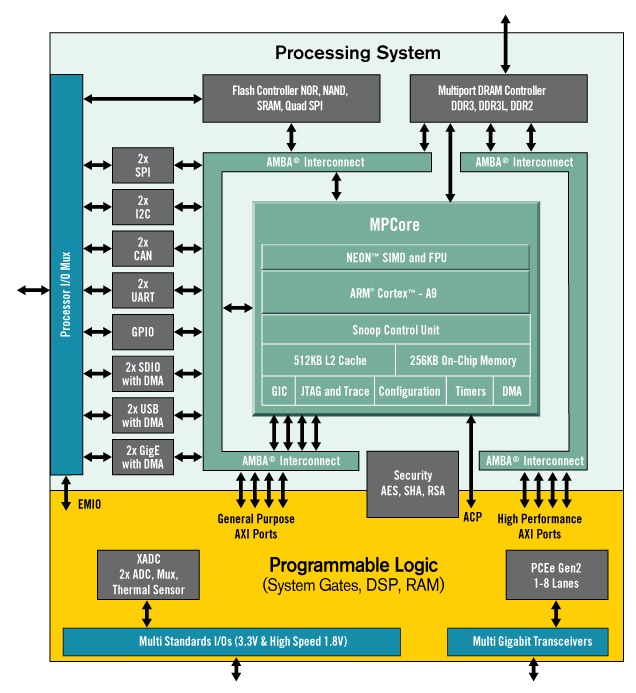
\includegraphics[scale=0.6]{obrazky-figures/zynq-mp-core-single.png}
						\caption{Architektura procesoru Zynq-7000\protect\footnotemark}
						\label{teorie::embedded::zynq}
					\end{center}
				\end{figure}
				\footnotetext{zdroj: \url{https://www.xilinx.com/products/silicon-devices/soc/zynq-7000.html}}
			
			\subsection{Řídící modul}
				Řídící modul obsahující výše zmíněný procesor je dodán společností CAMEA s.r.o. Modul obsahuje vstupně výstupní porty , které~můžeme využít v~náš prospěch. Jako výstupní porty můžeme využít USB sběrnici s~přímým přístupen do paměti, GPIO porty nebo Serial Peripheral Interface. 
				\begin{itemize}
					\item USB můžeme využít pro přenost přesných informací obrazovou formou na displej, kde zobrazujeme výšku. Formát by mohl být nasledující: \[ALTITUDE = 10.0 m\]\[ALTITUDE = 33 ft\]
					
					\item Pomocí GPIO portů, případně rozhraní SPI, můžeme ovládat panel s LE Diodami, který~barevnými LED seřazenými vertikálně. Tento panel bude mít diody vyzařující světlo od~zeleného spektra, přes žlutou, oranžovou a~sytě červenou, kdy~bude začínat fáze dosednutí.
					
					\item Zvuková komunikace může probíhat generováním tónů a~odesílání konektorem typu 3.5mm Jack. Bude se generovat stále stejný tón konstantní délky, přičemž zkracující se perioda bude signalizovat snižující se výšku. Pokud bude letadlo těsně nad zemí, bude se generovat tón bez přerušení.
				\end{itemize}
			
			\subsection{Kalibrace modulu}
				Další částí naší úlohy je nutnost kalibrace zařízení, jelikož každé letadlo může mít tento modul umístěno v jiné výšce nad zemí. Kalibrace může být statická - v kódu bude přičtena konstanta, nebo dynamická, kdy~se před startem modul zkalibruje. Statická kalibrace má výhodu jednoduššího chování modulu a~bude vyžadovat o~jeden ovládácí prvek méně, avšak bude nutno zasahovat do zdrojových kódů při instalaci na jiné letadlo. Dynamická kalibrace, narozdíl od~statické, má nevýhodu složitějšího řídícího programu, ale~je bude možno mít jeden program pro všechny typy letadel. Přidaný ovládácí prvek nebude téměř znát. V tomto případě se autor přiklání k~dynamické kalibraci.
				
			\subsection{Ovládací panel}
				Nutnost kalibrace nás přivádí k~ovládacímu panelu modulu. Přístroj je třeba nějak zapnout, toto bude první přepínač. Dále vyvstává otázka nutnosti mít vždy zapnutou zvukovou signalizaci. Jelikož bude využití tohoto výškoměru při vzletu mizivé, bude dobré, když~bude mít pilot možnost vypnout zvukovou indikaci, která~v~situaci, kdy~ji není potřeba může působit rušivě. Proto může být přítomen přepínač ovládající tuto funkci. Jako třetí kontrolní prvek zvolíme tlačítko spouštějící kalibraci přístroje na referenční hodnotu země. Je nutné, abychom zabránili kalibraci výškoměru ve vzduchu, proto by mělo toto tlačítko být překrité víčkem. V případě, že~bude koncipováno jako ovládací prvek na dotykovém displeji, za~pohybu letadla by mělo být deaktivované.
				
			
\chapter{Návrh řešení}\label{navrhReseni}
	Radarový výškoměr zpracovává vstupy zcela automaticky bez zásahu uživatele(pilota) a~uživateli pouze zobrazuje zpracované výsledky. Uživatel vůbec nepotřebuje vědět, co a~jak funguje, stačí mu pouze zobrazená výška. Vzhledem k~omezenému prostoru, kam~letadlo umožňuje instalovat další zařízení, jsme nuceni vyhledat co nejmenší řešení, které~je ale~zároveň dostatečně výkonné, aby~v~reálném čase zvládalo zpracovávat signály a~převést výsledky do vhodné formy pro rychlé a~správné vyhodnocení pilotem.
	
	\section{Hardware}\label{navrhReseni::hardware}
		\subsection{Radar}
			Radarový transciever, se~kterým~budeme v~této práci pracovat je K-MC1 Radar Transciever firmy RFbeam Microwave GmbH. Jedná se o kontinuálně vysílající a~příjmající radar s~frekvenční modulací. Díky frekvenční modulaci vysílaného signálu jsme schopni změřit nejenom rychlost objektu, ale~i~jeho vzdálenost, což je pro naše účely perfektní.
		
		\subsection{Výpočetní jednotka}\label{navrhReseni::hardware::vypocetniJednotka}
			Jak již bylo zmíněno v~úvodu této kapitoly, potřebujeme malé, ale~rychlé zařízení, které bude v~reálném čase poskytovat údaje o~aktuální výšce. V našem případě, vzhledem k~reakční době člověka cca půl sekundy, bude stačit, když systém stihne spočítat výsledek a~předat jej pilotovi do $\sim$250ms.\par
		
			Kvůli nárokům na velikost můžeme vyřadit objemné osobní počítače a~spíše se ponořit do~oblasti embedded systémů. V~současnosti trh nabízí dostatečně výkonné a~zároveň dostatečně kompaktní zařízení, která~jsou pro náš účel vhodná. Jako možný kandidát se jeví mikropočítač Raspberry Pi, který už je dostatečně výkonný a~zároveň malý aby mohl plnit naši úlohu. Vhodnější alternativa k~tomuto řešení se jeví procesor rodiny Zynq od~výrobce Xilinx, který je určen přesně pro naše potřeby, a~díky hradlovým polím FPGA výrazně urychluje zpracování ozvěny signálu. Přístroj s~procesorem dodala společnost CAMEA s.r.o.
		
		\subsection{Výstupní zařízení}
			Náš systém musí s~pilotem nějak komunikovat. Způsob komunikace musí být tak detailní, aby dokázal předat informace o~výšce nad~zemí a~zároveň dostatečně jednoduchý, aby pilot mohl data ze~systému zpracovat rychle a~efektivně aniž by výstupní zařízení odklánělo pozornost od~právě prováděných úkonů. Jedna z~možností je použití zvukových signálů, druhá je zobrazování aktuálních informací na displej. Autor se rozhodnul pro kombinaci obou způsobů. Zvukové signály umožní věnovat pozornost ději v~okolí letadla aniž by vyrušovaly pilota, pro podrobnější informace se bude moct podívat na displej.
			
	\section{Software}\label{navrhReseni::software}
		
		TODO %Poznamky autora, prosim nezlobte se. Linux, na kterem pobezi program tahajici data z radaru a pocitajici vyslednou vysku a rychlost, nutna konzultace na vystup zarizeni a testy co za cisla z toho vubec lezou, vysledek hratek s matlabem by se dal klasifikovat jako: meh. keywords: Hammingovo okno, 50\% prekryti vzorku => prace s poli => kastliku jak nasranych => program bude giganticky zrout pameti. Zjistit, jestli existuje knihovna pro praci se signaly v C at to nemusim prasit ja, bylo by to nefektivni a pomale.
	
	\section{Umístění na letadle}\label{navrhReseni::umisteniNaLetadle}
		Zařízení musí být na~letadle umístěno tak, ať~je šance požkození přístroje při tvrdším přistání minimální a~zároveň musí být měření konzistentní. Toto vylučuje umístění přístroje na~konci křídel. Může dojít k~odření křídla o~zem při přílišném naklonění, navíc bude muset být provedena velká korekce výšky a~může dojít k~změnám detekované výšky při náklonech letadla, taky dojde k narušení aerodynamického tvaru křídla. Ideální by bylo umístit senzor na pneumatiky jednoho z~kol hlavního podvozku, bohužel velice rychle zjistíme, že~je to nevhodné řešení z~důvodů jednorázového použití radaru. Jako vhodné možnosti se jeví umístění:
		\begin{itemize}
			\item na~nohu podvozku za předpokladu, že~se na~ni zařízení vejde(v případě zatažitelného podvozku). Při umístění na~pevný podvozek je třeba zamezit možnosti vzniku poškození následkem otřesů při tvrdém přistání. 
			\item na~spodní část kořene křídla, kde~nebude moment síly způsobující rotaci letadla ve~vodorovné ose tak velký, jako na konci křídla. Otřesy, které~bude muset zařízení snášet nebudou tak velké jako na noze hlavního podvozku. Bohužel zde zůstává nutnost korekce podle výšky kořene letadla nad~rovinou podvozku.
			\item na trup letadla, toto bohužel bude vyžadovat vrtání do trupu a~tudíž úpravu konstrukce letadla.
			\item do trupu letadla, ideálně do~odpružené schránky s~dvířky, která by se otevřela při spuštění radaru při náletu na přistání. Opět zde je otázka modifikace konstrukce letadla.
		\end{itemize} 
		Note: Asi bude nejlepší přilepit to na nohu, ať nemusíme vrtat, to je třeba zkonzultovat s majitelem letadla. Ostaní možnosti jsou příliš drahé.


%=========================================================================
 % viz. obsah.tex / see obsah.tex

  % Pouzita literatura / Bibliography
  % ----------------------------------------------
\ifslovak
  \makeatletter
  \def\@openbib@code{\addcontentsline{toc}{chapter}{Literatúra}}
  \makeatother
  \bibliographystyle{bib-styles/czechiso}
\else
  \ifczech
    \makeatletter
    \def\@openbib@code{\addcontentsline{toc}{chapter}{Literatura}}
    \makeatother
    \bibliographystyle{bib-styles/czechiso}
  \else 
    \makeatletter
    \def\@openbib@code{\addcontentsline{toc}{chapter}{Bibliography}}
    \makeatother
    \bibliographystyle{bib-styles/englishiso}
  %  \bibliographystyle{alpha}
  \fi
\fi
  \begin{flushleft}
  \bibliography{projekt-20-literatura-bibliography}
  \end{flushleft}

  % vynechani stranky v oboustrannem rezimu
  % Skip the page in the two-sided mode
  \iftwoside
    \cleardoublepage
  \fi

  % Prilohy / Appendices
  % ---------------------------------------------
  \appendix
\ifczech
  \renewcommand{\appendixpagename}{Přílohy}
  \renewcommand{\appendixtocname}{Přílohy}
  \renewcommand{\appendixname}{Příloha}
\fi
\ifslovak
  \renewcommand{\appendixpagename}{Prílohy}
  \renewcommand{\appendixtocname}{Prílohy}
  \renewcommand{\appendixname}{Príloha}
\fi
  \appendixpage

% vynechani stranky v oboustrannem rezimu
% Skip the page in the two-sided mode
\iftwoside
  \cleardoublepage
\fi
  
\ifslovak
%  \section*{Zoznam príloh}
%  \addcontentsline{toc}{section}{Zoznam príloh}
\else
  \ifczech
%    \section*{Seznam příloh}
%    \addcontentsline{toc}{section}{Seznam příloh}
  \else
%    \section*{List of Appendices}
%    \addcontentsline{toc}{section}{List of Appendices}
  \fi
\fi
  \startcontents[chapters]
  % seznam příloh / list of appendices
  % \printcontents[chapters]{l}{0}{\setcounter{tocdepth}{2}}
  
  % vynechani stranky v oboustrannem rezimu
  \iftwoside
    \cleardoublepage
  \fi
  %% Tento soubor nahraďte vlastním souborem s přílohami (nadpisy níže jsou pouze pro příklad)
%% This file should be replaced with your file with an appendices (headings below are examples only)
%
%% Umístění obsahu paměťového média do příloh je vhodné konzultovat s vedoucím
%% Placing of table of contents of the memory media here should be consulted with a supervisor
%%\chapter{Obsah přiloženého paměťového média}
%
%%\chapter{Manuál}
%
%%\chapter{Konfigurační soubor} % Configuration file
%
%%\chapter{RelaxNG Schéma konfiguračního souboru} % Scheme of RelaxNG configuration file
%
%%\chapter{Plakát} % poster
%
%\chapter{Jak pracovat s touto šablonou}
%\label{jak}
%
%V této kapitole je uveden popis jednotlivých částí šablony, po kterém následuje stručný návod, jak s touto šablonou pracovat. 
%
%Jedná se o přechodnou verzi šablony. Nová verze bude zveřejněna do konce roku 2016 a bude navíc obsahovat nové pokyny ke správnému využití šablony, závazné pokyny k~vypracování bakalářských a diplomových prací (rekapitulace pokynů, které jsou dostupné na~webu) a nezávazná doporučení od vybraných vedoucích. Jediné soubory, které se v nové verzi změní, budou projekt-01-kapitoly-chapters.tex a projekt-30-prilohy-appendices.tex, jejichž obsah každý student vymaže a nahradí vlastním. Šablonu lze tedy bez problémů využít i~v~současné verzi.
%
%\section*{Popis částí šablony}
%
%Po rozbalení šablony naleznete následující soubory a adresáře:
%\begin{DESCRIPTION}
%  \item [bib-styles] Styly literatury (viz níže). 
%  \item [obrazky-figures] Adresář pro Vaše obrázky. Nyní obsahuje placeholder.pdf (tzv. TODO obrázek, který lze použít jako pomůcku při tvorbě technické zprávy), který se s prací neodevzdává. Název adresáře je vhodné zkrátit, aby byl jen ve zvoleném jazyce.
%  \item [template-fig] Obrázky šablony (znak VUT).
%  \item [fitthesis.cls] Šablona (definice vzhledu).
%  \item [Makefile] Makefile pro překlad, počítání normostran, sbalení apod. (viz níže).
%  \item [projekt-01-kapitoly-chapters.tex] Soubor pro Váš text (obsah nahraďte).
%  \item [projekt-20-literatura-bibliography.bib] Seznam literatury (viz níže).
%  \item [projekt-30-prilohy-appendices.tex] Soubor pro přílohy (obsah nahraďte).
%  \item [projekt.tex] Hlavní soubor práce -- definice formálních částí.
%\end{DESCRIPTION}
%
%Výchozí styl literatury (czechiso) je od Ing. Martínka, přičemž anglická verze (englishiso) je jeho překladem s drobnými modifikacemi. Oproti normě jsou v něm určité odlišnosti, ale na FIT je dlouhodobě akceptován. Alternativně můžete využít styl od Ing. Radima Loskota nebo od Ing. Radka Pyšného\footnote{BP Ing. Radka Pyšného \url{http://www.fit.vutbr.cz/study/DP/BP.php?id=7848}}. Alternativní styly obsahují určitá vylepšení, ale zatím nebyly řádně otestovány větším množstvím uživatelů. Lze je považovat za beta verze pro zájemce, kteří svoji práci chtějí mít dokonalou do detailů a neváhají si nastudovat detaily správného formátování citací, aby si mohli ověřit, že je vysázený výsledek v pořádku.
%
%Makefile kromě překladu do PDF nabízí i další funkce:
%\begin{itemize}
%  \item přejmenování souborů (viz níže),
%  \item počítání normostran,
%  \item spuštění vlny pro doplnění nezlomitelných mezer,
%  \item sbalení výsledku pro odeslání vedoucímu ke kontrole (zkontrolujte, zda sbalí všechny Vámi přidané soubory, a případně doplňte).
%\end{itemize}
%
%Nezapomeňte, že vlna neřeší všechny nezlomitelné mezery. Vždy je třeba manuální kontrola, zda na konci řádku nezůstalo něco nevhodného -- viz Internetová jazyková příručka\footnote{Internetová jazyková příručka \url{http://prirucka.ujc.cas.cz/?id=880}}.
%
%\paragraph {Pozor na číslování stránek!} Pokud má obsah 2 strany a na 2. jsou jen \uv{Přílohy} a~\uv{Seznam příloh} (ale žádná příloha tam není), z nějakého důvodu se posune číslování stránek o 1 (obsah \uv{nesedí}). Stejný efekt má, když je na 2. či 3. stránce obsahu jen \uv{Literatura} a~je možné, že tohoto problému lze dosáhnout i jinak. Řešení je několik (od~úpravy obsahu, přes nastavení počítadla až po sofistikovanější metody). \textbf{Před odevzdáním proto vždy překontrolujte číslování stran!}
%
%
%\section*{Doporučený postup práce se šablonou}
%
%\begin{enumerate}
%  \item \textbf{Zkontrolujte, zda máte aktuální verzi šablony.} Máte-li šablonu z předchozího roku, na stránkách fakulty již může být novější verze šablony s~aktualizovanými informacemi, opravenými chybami apod.
%  \item \textbf{Zvolte si jazyk}, ve kterém budete psát svoji technickou zprávu (česky, slovensky nebo anglicky) a svoji volbu konzultujte s vedoucím práce (nebyla-li dohodnuta předem). Pokud Vámi zvoleným jazykem technické zprávy není čeština, nastavte příslušný parametr šablony v souboru projekt.tex (např.: \verb|documentclass[english]{fitthesis}| a přeložte prohlášení a poděkování do~angličtiny či slovenštiny.
%  \item \textbf{Přejmenujte soubory.} Po rozbalení je v šabloně soubor projekt.tex. Pokud jej přeložíte, vznikne PDF s technickou zprávou pojmenované projekt.pdf. Když vedoucímu více studentů pošle projekt.pdf ke kontrole, musí je pracně přejmenovávat. Proto je vždy vhodné tento soubor přejmenovat tak, aby obsahoval Váš login a (případně zkrácené) téma práce. Vyhněte se však použití mezer, diakritiky a speciálních znaků. Vhodný název tedy může být např.: \uv{xlogin00-Cisteni-a-extrakce-textu.tex}. K přejmenování můžete využít i přiložený Makefile:
%\begin{verbatim}
%make rename NAME=xlogin00-Cisteni-a-extrakce-textu
%\end{verbatim}
%  \item Vyplňte požadované položky v souboru, který byl původně pojmenován projekt.tex, tedy typ, rok (odevzdání), název práce, svoje jméno, ústav (dle zadání), tituly a~jméno vedoucího, abstrakt, klíčová slova a další formální náležitosti.
%  \item Nahraďte obsah souborů s kapitolami práce, literaturou a přílohami obsahem svojí technické zprávy. Jednotlivé přílohy či kapitoly práce může být výhodné uložit do~samostatných souborů -- rozhodnete-li se pro toto řešení, je doporučeno zachovat konvenci pro názvy souborů, přičemž za číslem bude následovat název kapitoly. 
%  \item Nepotřebujete-li přílohy, zakomentujte příslušnou část v projekt.tex a příslušný soubor vyprázdněte či smažte. Nesnažte se prosím vymyslet nějakou neúčelnou přílohu jen proto, aby daný soubor bylo čím naplnit. Vhodnou přílohou může být obsah přiloženého paměťového média.
%  \item Nascanované zadání uložte do souboru zadani.pdf a povolte jeho vložení do práce parametrem šablony v projekt.tex (\verb|documentclass[zadani]{fitthesis}|).
%  \item Nechcete-li odkazy tisknout barevně (tedy červený obsah -- bez konzultace s vedoucím nedoporučuji), budete pro tisk vytvářet druhé PDF s tím, že nastavíte parametr šablony pro tisk: (\verb|documentclass[zadani,print]{fitthesis}|).  Barevné logo se nesmí tisknout černobíle!
%  \item Vzor desek, do kterých bude práce vyvázána, si vygenerujte v informačním systému fakulty u zadání. Pro disertační práci lze zapnout parametrem v šabloně (více naleznete v souboru fitthesis.cls).
%  \item Nezapomeňte, že zdrojové soubory i (obě verze) PDF musíte odevzdat na CD či jiném médiu přiloženém k technické zprávě.
%\end{enumerate}
%
%\subsection*{Pokyny pro oboustranný tisk}
%\begin{itemize}
%\item Zapíná se parametrem šablony: \verb|\documentclass[twoside]{fitthesis}|
%\item Po vytištění oboustranného listu zkontrolujte, zda je při prosvícení sazební obrazec na obou stranách na stejné pozici. Méně kvalitní tiskárny s duplexní jednotkou mají často posun o 1--3 mm. Toto může být u některých tiskáren řešitelné tak, že vytisknete nejprve liché stránky, pak je dáte do stejného zásobníku a vytisknete sudé.
%\item Za titulním listem, obsahem, literaturou, úvodním listem příloh, seznamem příloh a případnými dalšími seznamy je třeba nechat volnou stránku, aby následující část začínala na liché stránce (\textbackslash cleardoublepage).
%\item  Konečný výsledek je nutné pečlivě překontrolovat.
%\end{itemize}
%
%
%\subsection*{Užitečné nástroje}
%\label{nastroje}
%
%Následující seznam není výčtem všech využitelných nástrojů. Máte-li vyzkoušený osvědčený nástroj, neváhejte jej využít. Pokud však nevíte, který nástroj si zvolit, můžete zvážit některý z následujících:
%
%\begin{description}
%	\item[\href{http://miktex.org/download}{MikTeX}] \LaTeX{} pro Windows -- distribuce s jednoduchou instalací a vynikající automatizací stahování balíčků.
%	\item[\href{http://texstudio.sourceforge.net/}{TeXstudio}] Přenositelné opensource GUI pro \LaTeX{}.  Ctrl+klik umožňuje přepínat mezi zdrojovým textem a PDF. Má integrovanou kontrolu pravopisu, zvýraznění syntaxe apod. Pro jeho využití je nejprve potřeba nainstalovat MikTeX.
%	\item[\href{http://jabref.sourceforge.net/download.php}{JabRef}] Pěkný a jednoduchý program v Javě pro správu souborů s bibliografií (literaturou). Není potřeba se nic učit -- poskytuje jednoduché okno a formulář pro editaci položek.
%	\item[\href{https://inkscape.org/en/download/}{InkScape}] Přenositelný opensource editor vektorové grafiky (SVG i PDF). Vynikající nástroj pro tvorbu obrázků do odborného textu. Jeho ovládnutí je obtížnější, ale výsledky stojí za to.
%	\item[\href{https://git-scm.com/}{GIT}] Vynikající pro týmovou spolupráci na projektech, ale může výrazně pomoci i jednomu autorovi. Umožňuje jednoduché verzování, zálohování a přenášení mezi více počítači.
%	\item[\href{http://www.overleaf.com/}{Overleaf}] Online nástroj pro \LaTeX{}. Přímo zobrazuje náhled a umožňuje jednoduchou spolupráci (vedoucí může průběžně sledovat psaní práce), vyhledávání ve zdrojovém textu kliknutím do PDF, kontrolu pravopisu apod. Zdarma jej však lze využít pouze s určitými omezeními (někomu stačí na disertaci, jiný na ně může narazit i při psaní bakalářské práce) a pro dlouhé texty je pomalejší.
%\end{description}
%
%\subsection*{Užitečné balíčky pro \LaTeX}
%
%Studenti při sazbě textu často řeší stejné problémy. Některé z nich lze vyřešit následujícími balíčky pro \LaTeX:
%
%\begin{itemize}
%  \item \verb|amsmath| -- rozšířené možnosti sazby rovnic,
%  \item \verb|float, afterpage, placeins| -- úprava umístění obrázků,
%  \item \verb|fancyvrb, alltt| -- úpravy vlastností prostředí Verbatim, 
%  \item \verb|makecell| -- rozšíření možností tabulek,
%  \item \verb|pdflscape, rotating| -- natočení stránky o 90 stupňů (pro obrázek či tabulku),
%  \item \verb|hyphenat| -- úpravy dělení slov,
%  \item \verb|picture, epic, eepic| -- přímé kreslení obrázků.
%\end{itemize}
%
%Některé balíčky jsou využity přímo v šabloně (v dolní části souboru fitthesis.cls). Nahlédnutí do jejich dokumentace může být rovněž užitečné.
%
%Sloupec tabulky zarovnaný vlevo s pevnou šířkou je v šabloně definovaný \uv{L} (používá se jako \uv{p}).
%
 % viz. prilohy.tex / see prilohy.tex
\end{document}
